\documentclass[a4paper,12pt]{article}
\usepackage[utf8]{inputenc}
\usepackage[english]{babel}
\usepackage{amsmath,amsfonts,amssymb}
\usepackage{graphicx}
\usepackage{caption}
\usepackage{hyperref}
\usepackage{geometry}
\usepackage{booktabs}
\usepackage[separate-uncertainty=true]{siunitx} % SI-Einheiten
\usepackage{float}
\usepackage[ISO]{diffcoeff} % Differentiale in hübsch
\usepackage{subcaption} % Bilder nebeneinander
\usepackage{wrapfig} % Bilder und Text zusammen
\usepackage{enumitem}
\usepackage{physics}
\usepackage[table]{xcolor}

\geometry{left=2.5cm, right=2.5cm, top=2.5cm, bottom=2.5cm}

\title{Update: SIMBA in python}
\author{Stella Hoffmann}
\date{March}

\begin{document}

\maketitle

\tableofcontents

\newpage

\section{What I did}
\begin{figure}[H]
    \centering
    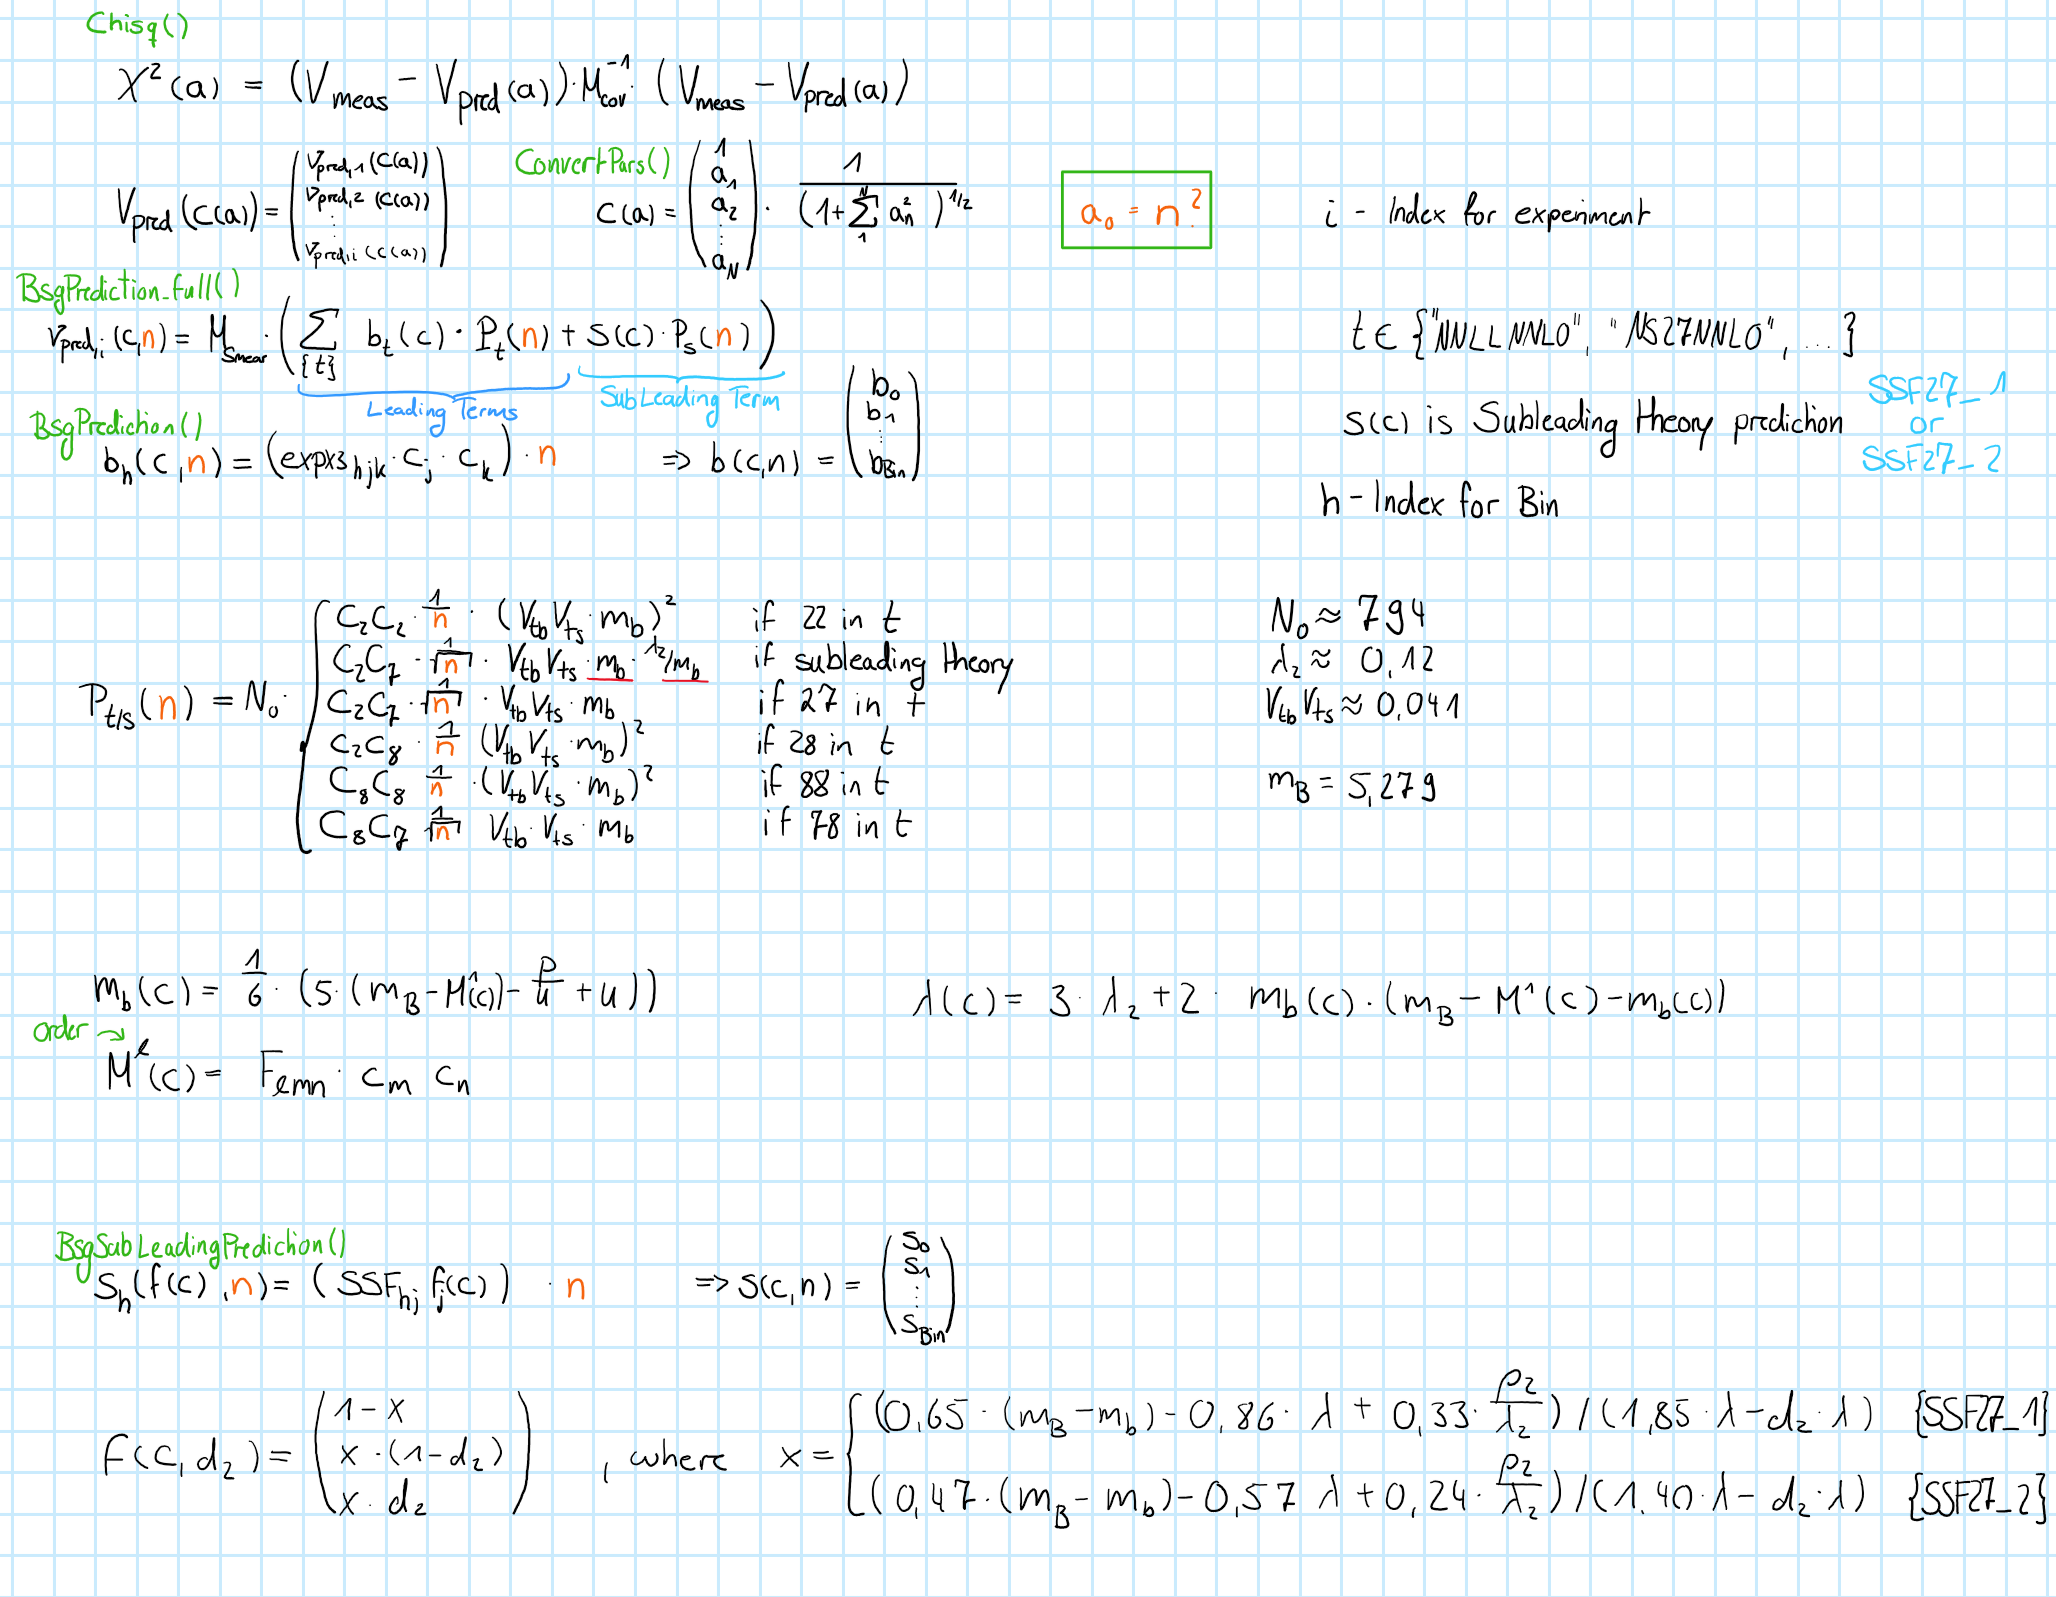
\includegraphics[scale=0.3]{equations.png}
    \caption{Equations according to my python code}
\end{figure}

A problem could be the $d_2$. In my code it's constantly zero. I got this information from the \textit{fit.config} file.
\begin{figure}[H]
    \centering
    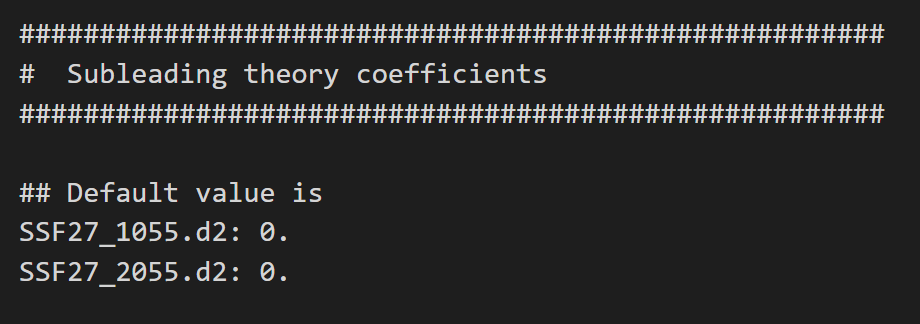
\includegraphics[scale=0.3]{d2_fit_config.png}
    \caption{Information in \textit{fit.config} file}
\end{figure}

\section{Comparisons}
As you can see in the following, something is off with the subleading theory. To compare different fits, I always plotted the Fit with the subleading prediction added on the leading prediction and with just the leading prediction.
For the fitting I used 4 to 7 start parameters, which gave different results for the prediction, as it is shown in the columns.
Every pair of rows has more amount of measurements included in the fit (\textit{["babar\_incl", "babar\_hadtag", "babar\_sem", "belle"]}).\\
\subsection{Results for each fit}
In the tables and in the following figueres, I circled the best looking fit green. The best looking fit was the one with the lowest $\chi^2$ and the $m_b$ which was closest to the result from the paper, which is listet in the first table in the last row.
The best looking fit is without the subleading theory, and looks good for the first two measurements (\textit{"babar\_incl", "babar\_hadtag"}) but for the third (\textit{"babar\_sem"}) it starts to differ a lot from the aimed fit.
\begin{table}[H]
    \begin{tabular}{|p{3.5cm}|p{3.5cm}|p{3.5cm}|l|l|l|}
        \hline
        Number of included measurements & With or without subleading theory & Number of fitted parameters & $\chi^2$ & $m_b$ [\unit{GeV}] & $a_0$ (Norm) \\
        \hline
        2&subleading&4&174477.25&4.6877&0.9204\\
        2&subleading&5&143976.56&4.6900&0.9514\\
        2&subleading&6&145631.54&4.6843&0.9678\\
        2&subleading&7&248645.38&4.5712&0.9708\\
        2&leading&4&230.97&4.6932&0.3826\\
        2&leading&5&323.33&4.8005&0.5210\\
        2&leading&6&262.79&4.8515&0.5774\\
        2&leading&7&292.88&4.1603&0.6252\\
        3&subleading&4&91211.26&4.6821&0.9228\\
        3&subleading&5&67852.28&4.6845&0.9519\\
        3&subleading&6&66673.56&4.6711&0.9680\\
        3&subleading&7&139735.90&4.5526&0.9721\\
        3&leading&4&167.13&3.9984&0.5020\\
        3&leading&5&258.61&4.7932&0.4933\\
        3&leading&6&156.92&3.9980&0.8149\\
        3&leading&7&231.09&4.7644&0.2352\\
        4&subleading&4&45178.57&4.7032&0.9143\\
        4&subleading&5&19.59&3.4633&0.0426\\
        4&subleading&6&23165.42&4.7386&0.9323\\
        4&subleading&7&22746.34&4.5274&0.9208\\
        4&leading&4&12.36&4.5904&0.4373\\
        4&leading&5&11.72&4.4835&0.6715\\
        \rowcolor{green!20} % 20 % hellgrün
        4&leading&6&10.10&4.7076&0.3762\\
        4&leading&7&14.15&4.2259&0.0892\\
        \hline
        \hline
        Result from paper&&&&4.764&\\
        \hline 
    \end{tabular}
    \caption{Values calculated with the fit-parameters}
\end{table}

\begin{table}[H]
    \begin{tabular}{|l|l|l|l|l|l|l|l|l|l|l|}
        \hline
        $n_{meas}$&&$n_{pars}$&$c_0$ & $c_1$& $c_2$ & $c_3$ & $c_4$ & $c_5$ & $c_6$\\
        \hline
        2&s&4&0.896&-0.394&0.159&0.126\\
        2&s&5&0.855&-0.438&0.181&0.182&0.102\\
        2&s&6&0.842&-0.450&0.183&0.203&0.121&0.011\\
        2&s&7&0.709&-0.101&-0.205&0.625&-0.107&0.184&-0.096\\
        2&l&4&0.890&-0.441&0.009&0.113\\
        2&l&5&0.025&-0.089&0.758&-0.646&-0.023\\
        2&l&6&0.032&0.043&0.284&-0.739&0.608&0.020\\
        2&l&7&0.000&-0.494&0.524&0.457&0.496&0.153&-0.058\\
        3&s&4&0.910&-0.378&0.139&0.095\\
        3&s&5&0.867&-0.422&0.176&0.169&0.098\\
        3&s&6&0.852&-0.433&0.174&0.200&0.123&0.030\\
        3&s&7&0.742&-0.153&-0.116&0.599&-0.097&0.178&-0.115\\
        3&l&4&0.000&0.880&0.473&-0.033\\
        3&l&5&0.032&-0.090&0.642&-0.760&-0.018\\
        3&l&6&0.000&0.815&0.568&-0.110&0.019&0.001\\
        3&l&7&0.000&0.371&-0.061&0.489&-0.775&0.053&0.126\\
        4&s&4&0.857&-0.433&0.214&0.178\\
        4&s&5&0.022&0.587&0.531&0.494&0.358\\
        4&s&6&0.242&-0.178&0.812&-0.387&0.062&0.310\\
        4&s&7&0.132&0.431&-0.225&0.589&0.300&-0.438&0.343\\
        4&l&4&0.231&0.391&-0.891&-0.017\\
        4&l&5&0.148&-0.163&0.974&0.055&-0.005\\
        \rowcolor{green!20} % 20 % hellgrün
        4&l&6&0.034&0.875&-0.445&0.107&-0.096&-0.122\\
        4&l&7&0.019&0.297&0.117&-0.089&0.062&-0.907&-0.251\\
        \hline
    \end{tabular}
    \caption{$c_n$ calculated by $a_n$ which are the fitted parameters}
\end{table}
\noindent In the following:
The \textbf{red dots} show my calculated prediction.\\
The \textbf{black dots} show the experimental values, which I extracted from the root files.\\
The \textbf{green line} shows the fit I extracted from the root files.\\
The \textbf{blue line} shows the difference between the green line and the red dots.
\subsection{Babar hadronic tag}
\begin{figure}[H]
    \centering
    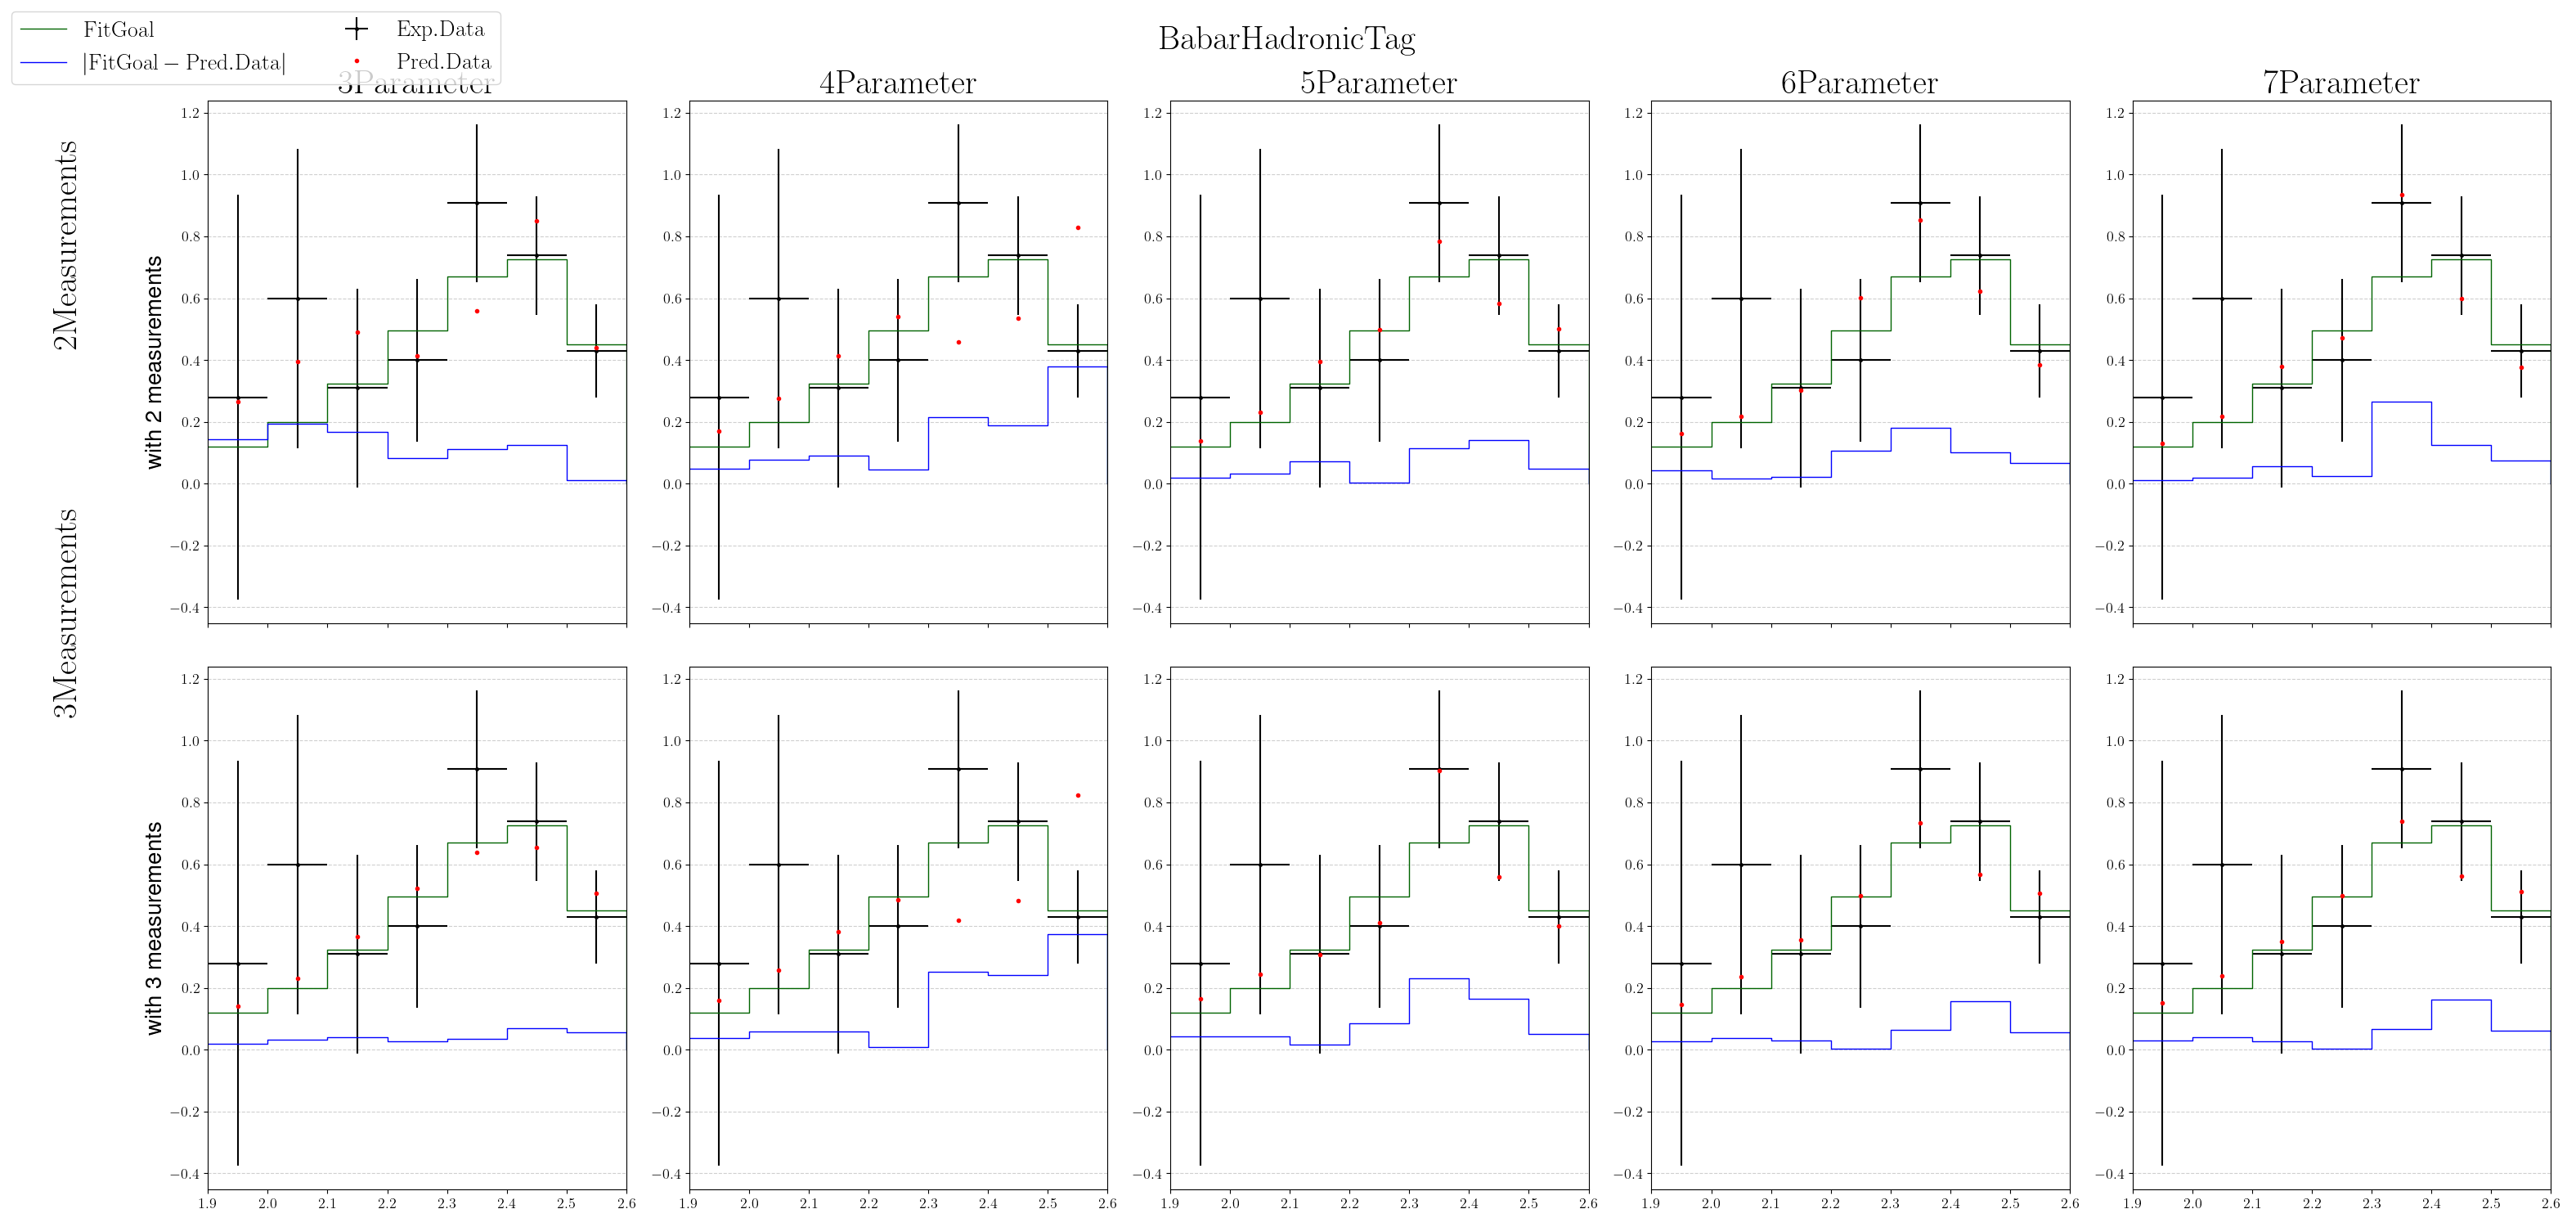
\includegraphics[scale=0.3]{../compare/babar_hadtag_soft_compare.png}
    \caption{Fit Comparison for 'babar\_hadtag'}
\end{figure}
\subsection{Babar inclusive spectra}
\begin{figure}[H]
    \centering
    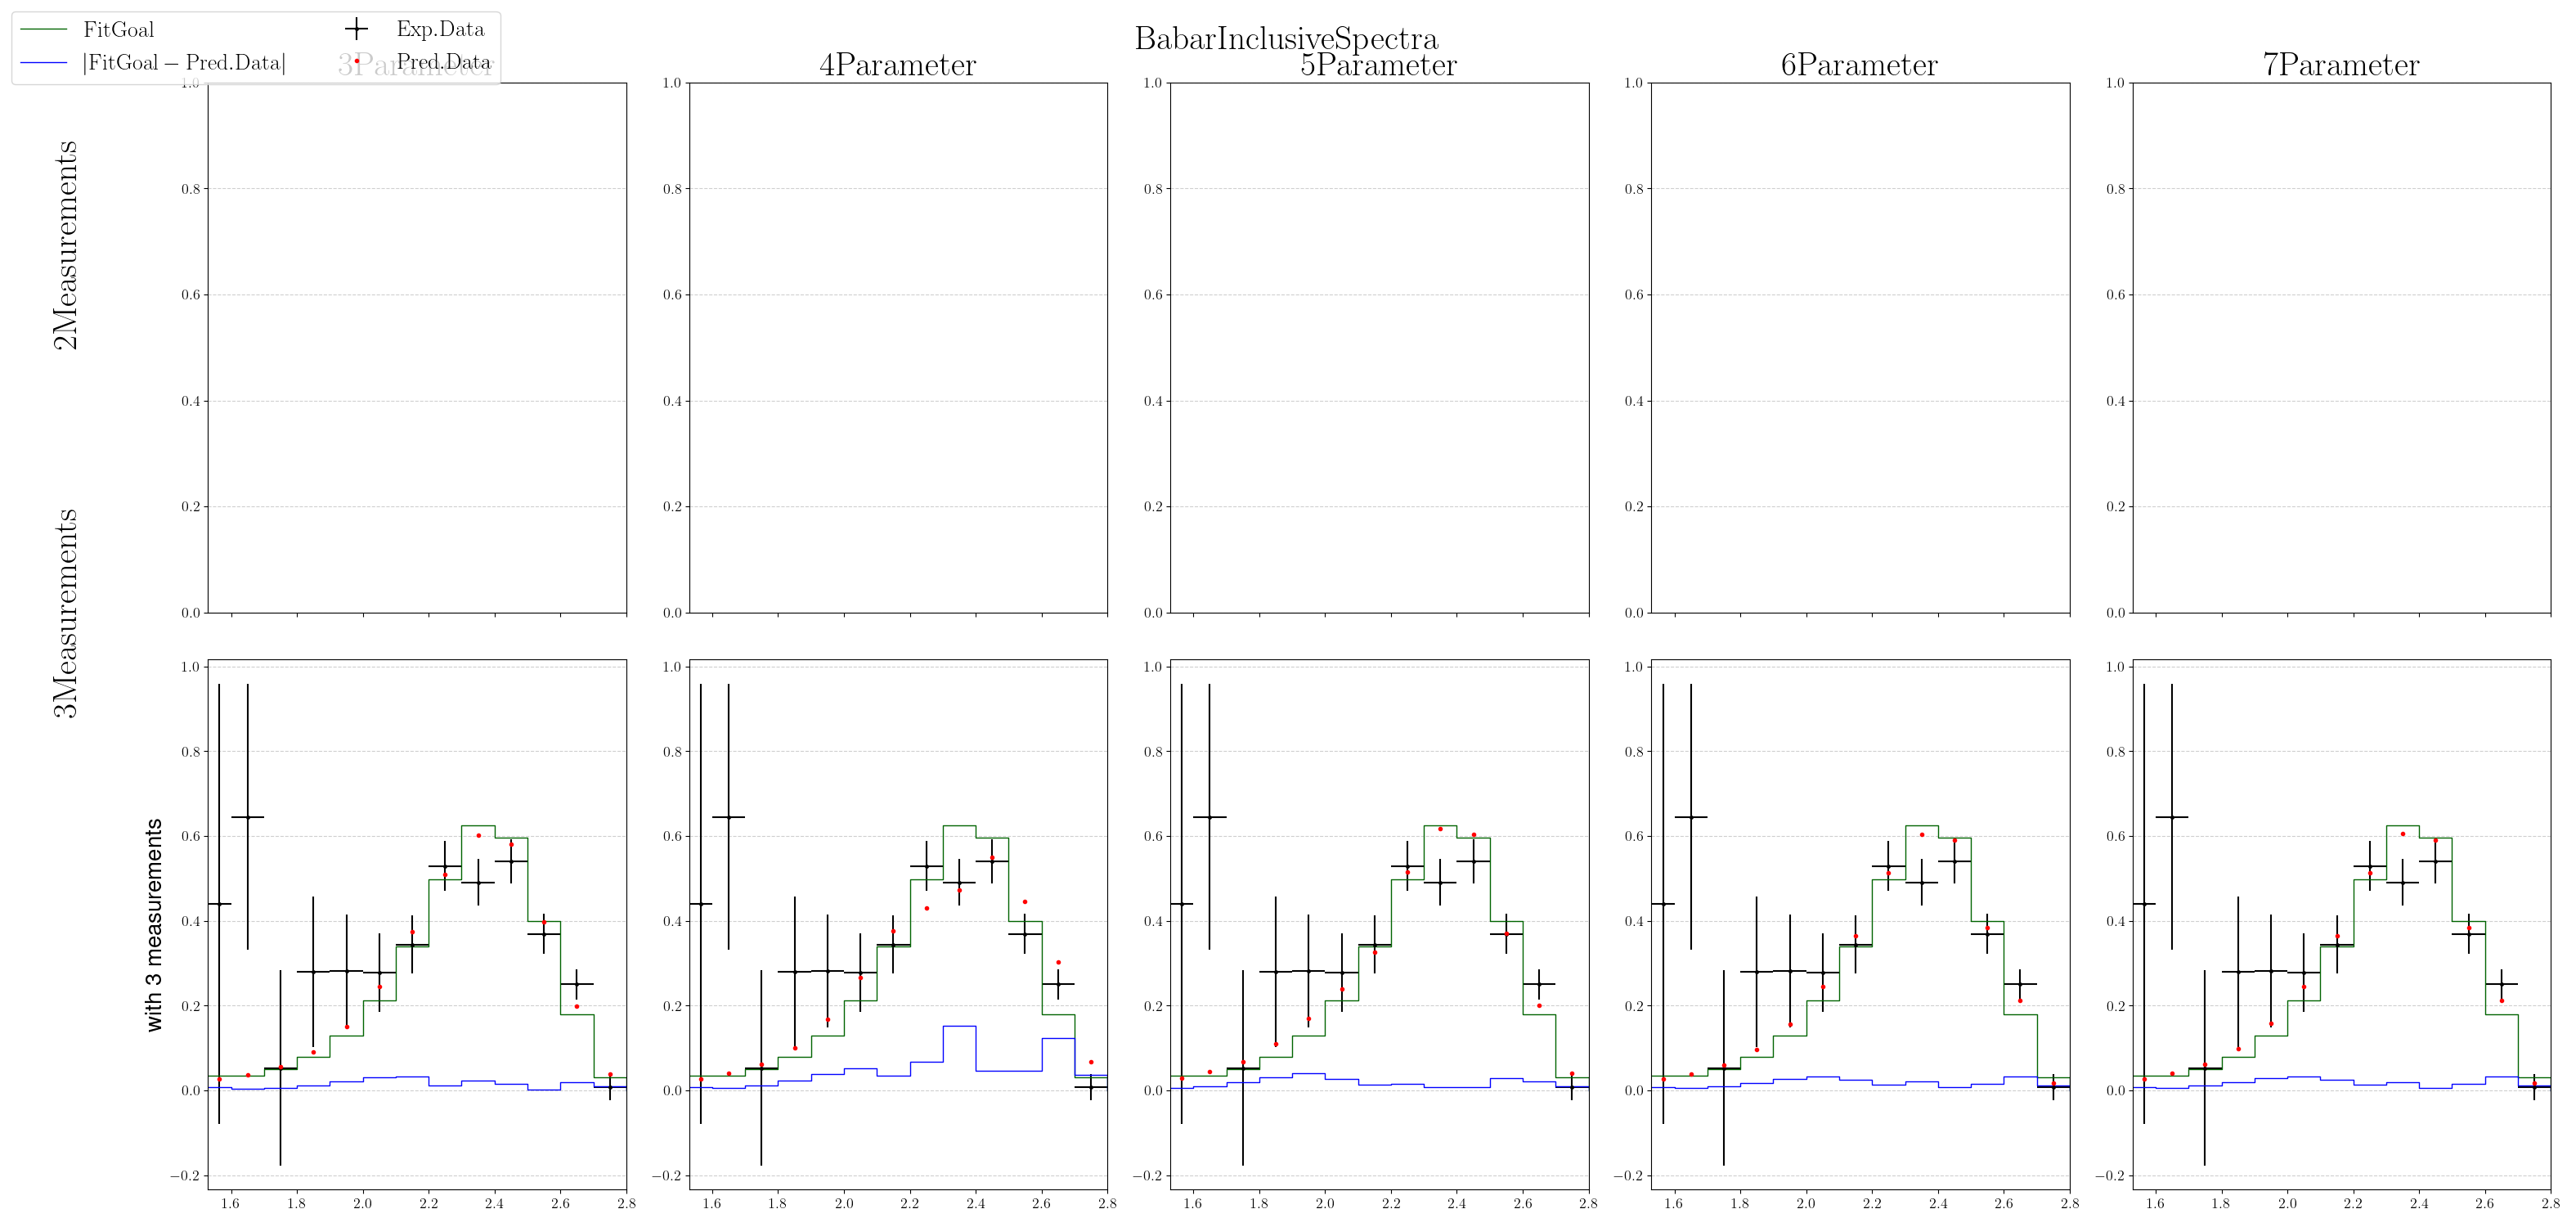
\includegraphics[scale=0.3]{../compare/babar_incl_soft_compare.png}
    \caption{Fit Comparison for 'babar\_incl'}
\end{figure}
\subsection{Babar semileptonic}
\begin{figure}[H]
    \centering
    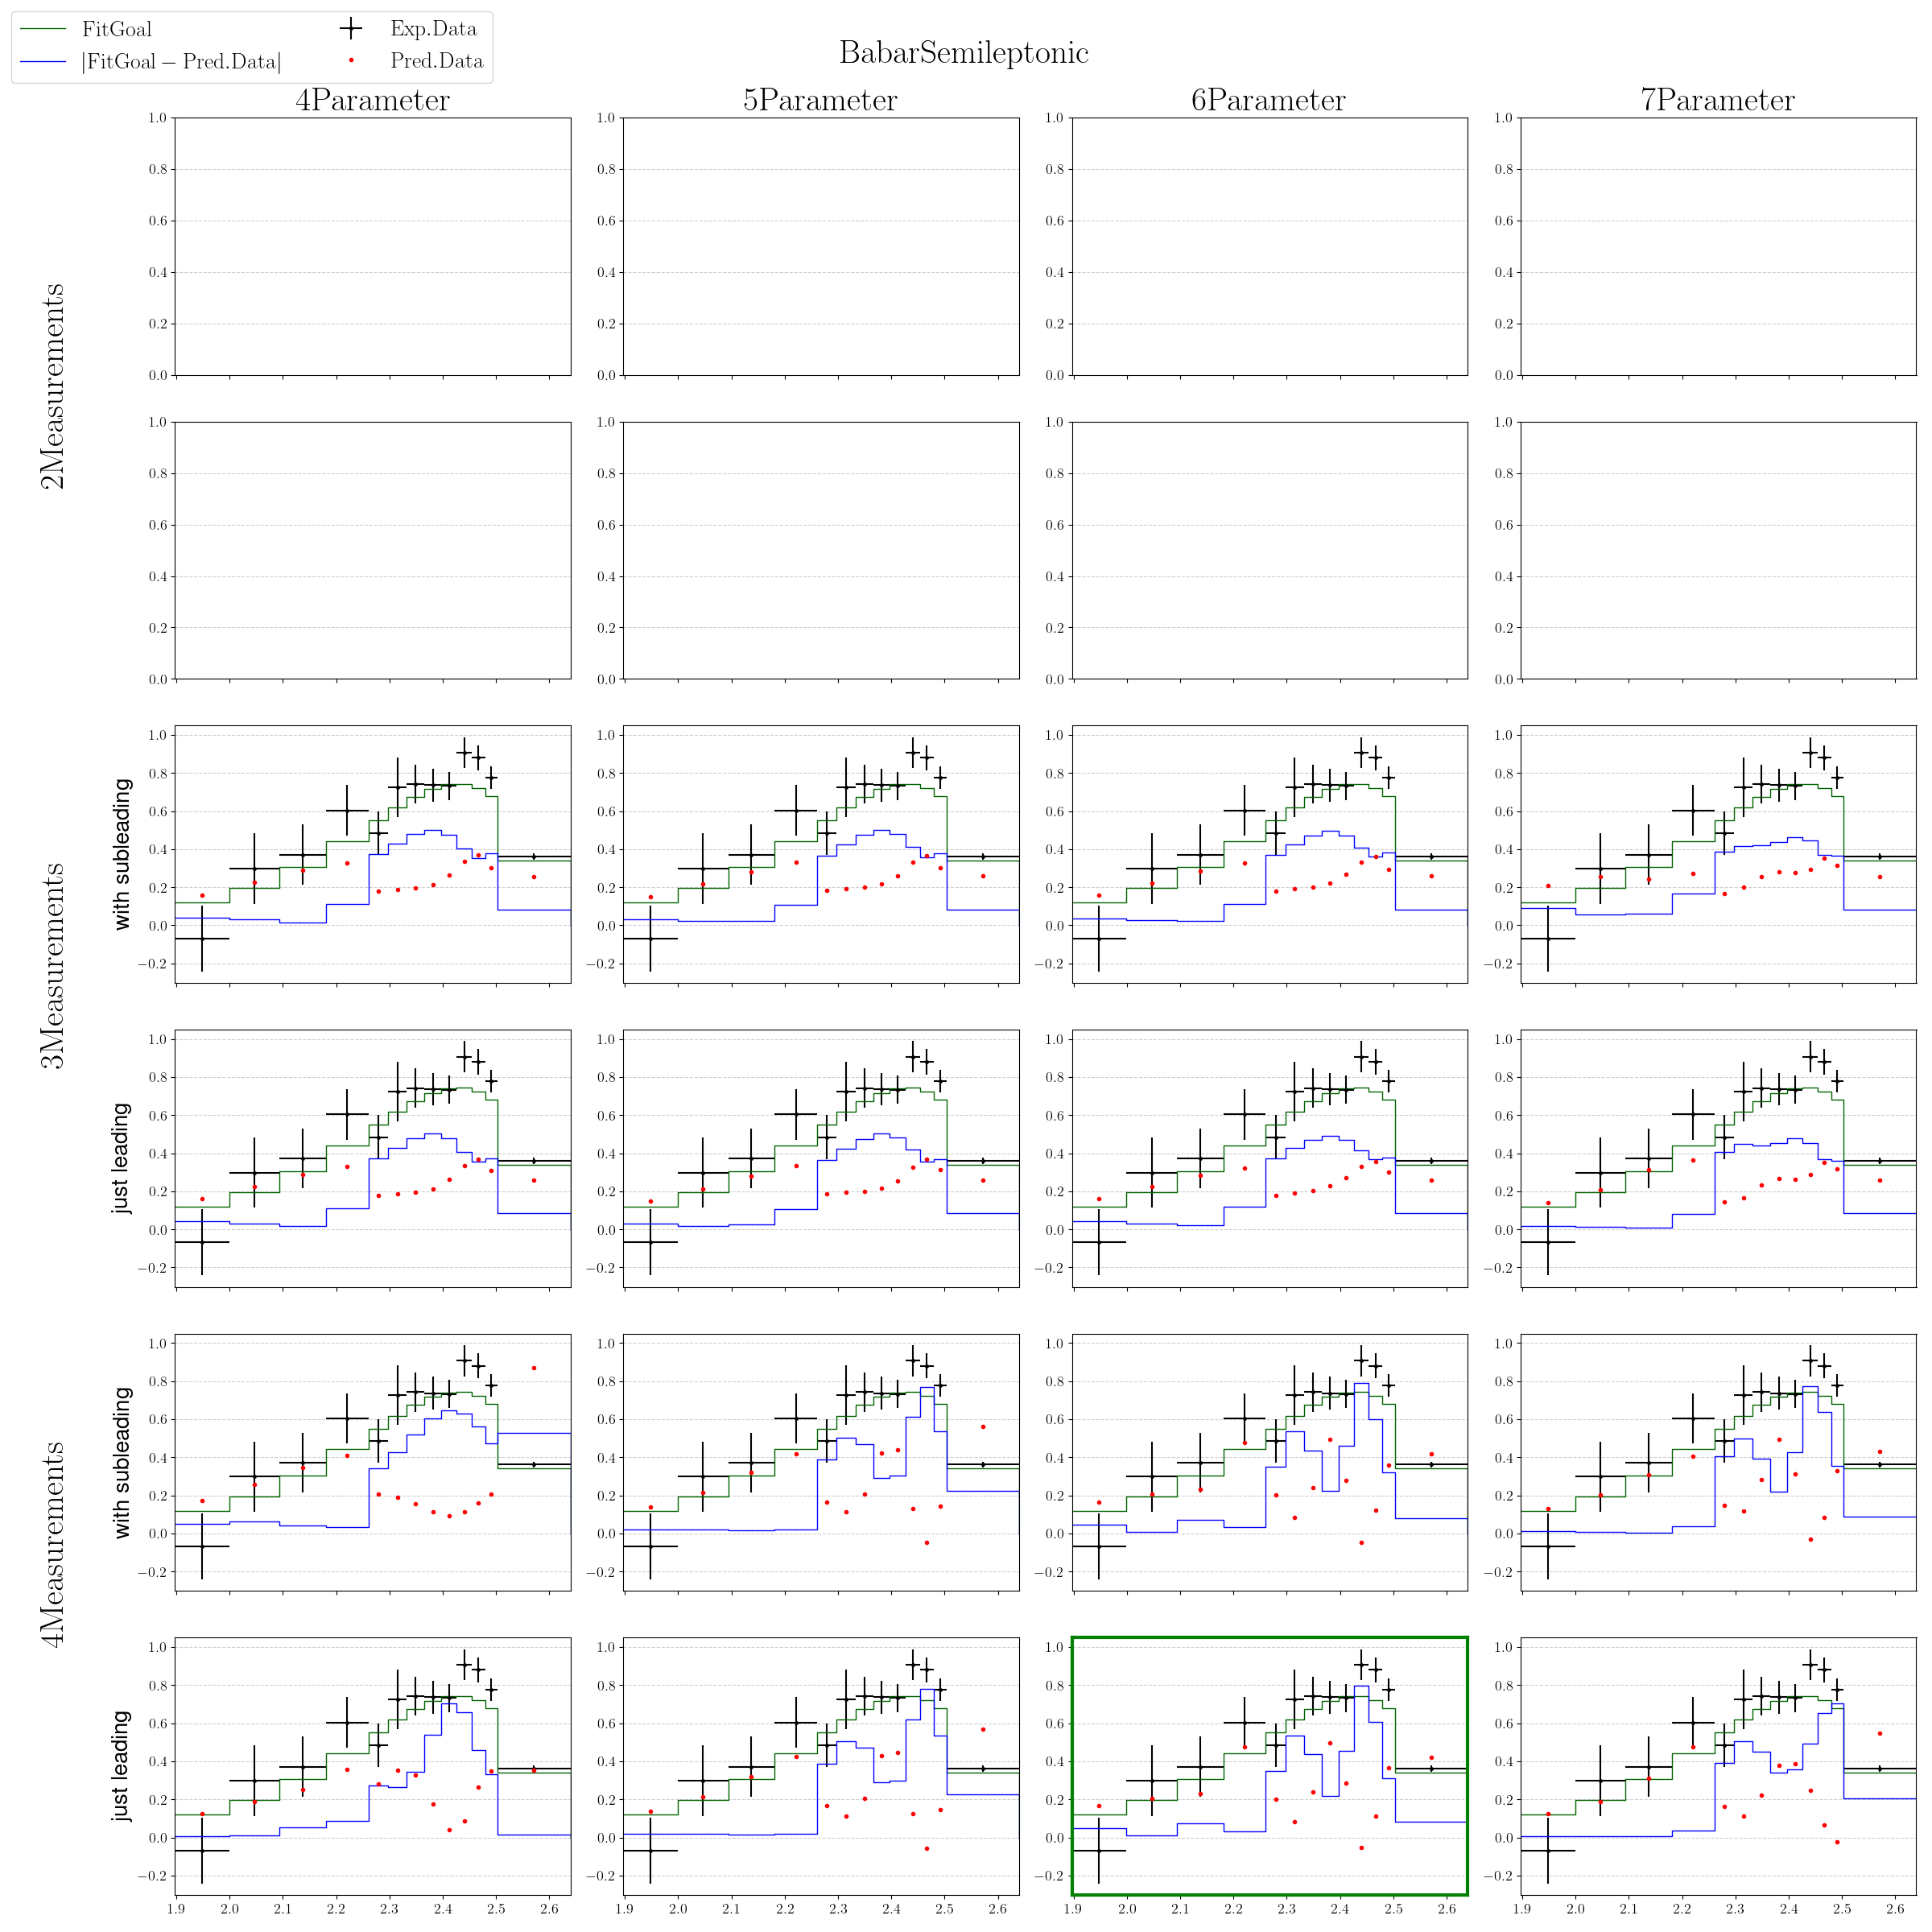
\includegraphics[scale=0.3]{../compare/babar_sem_soft_compare.png}
    \caption{Fit Comparison for 'babar\_sem'}
\end{figure}
\subsection{Belle}
\begin{figure}[H]
    \centering
    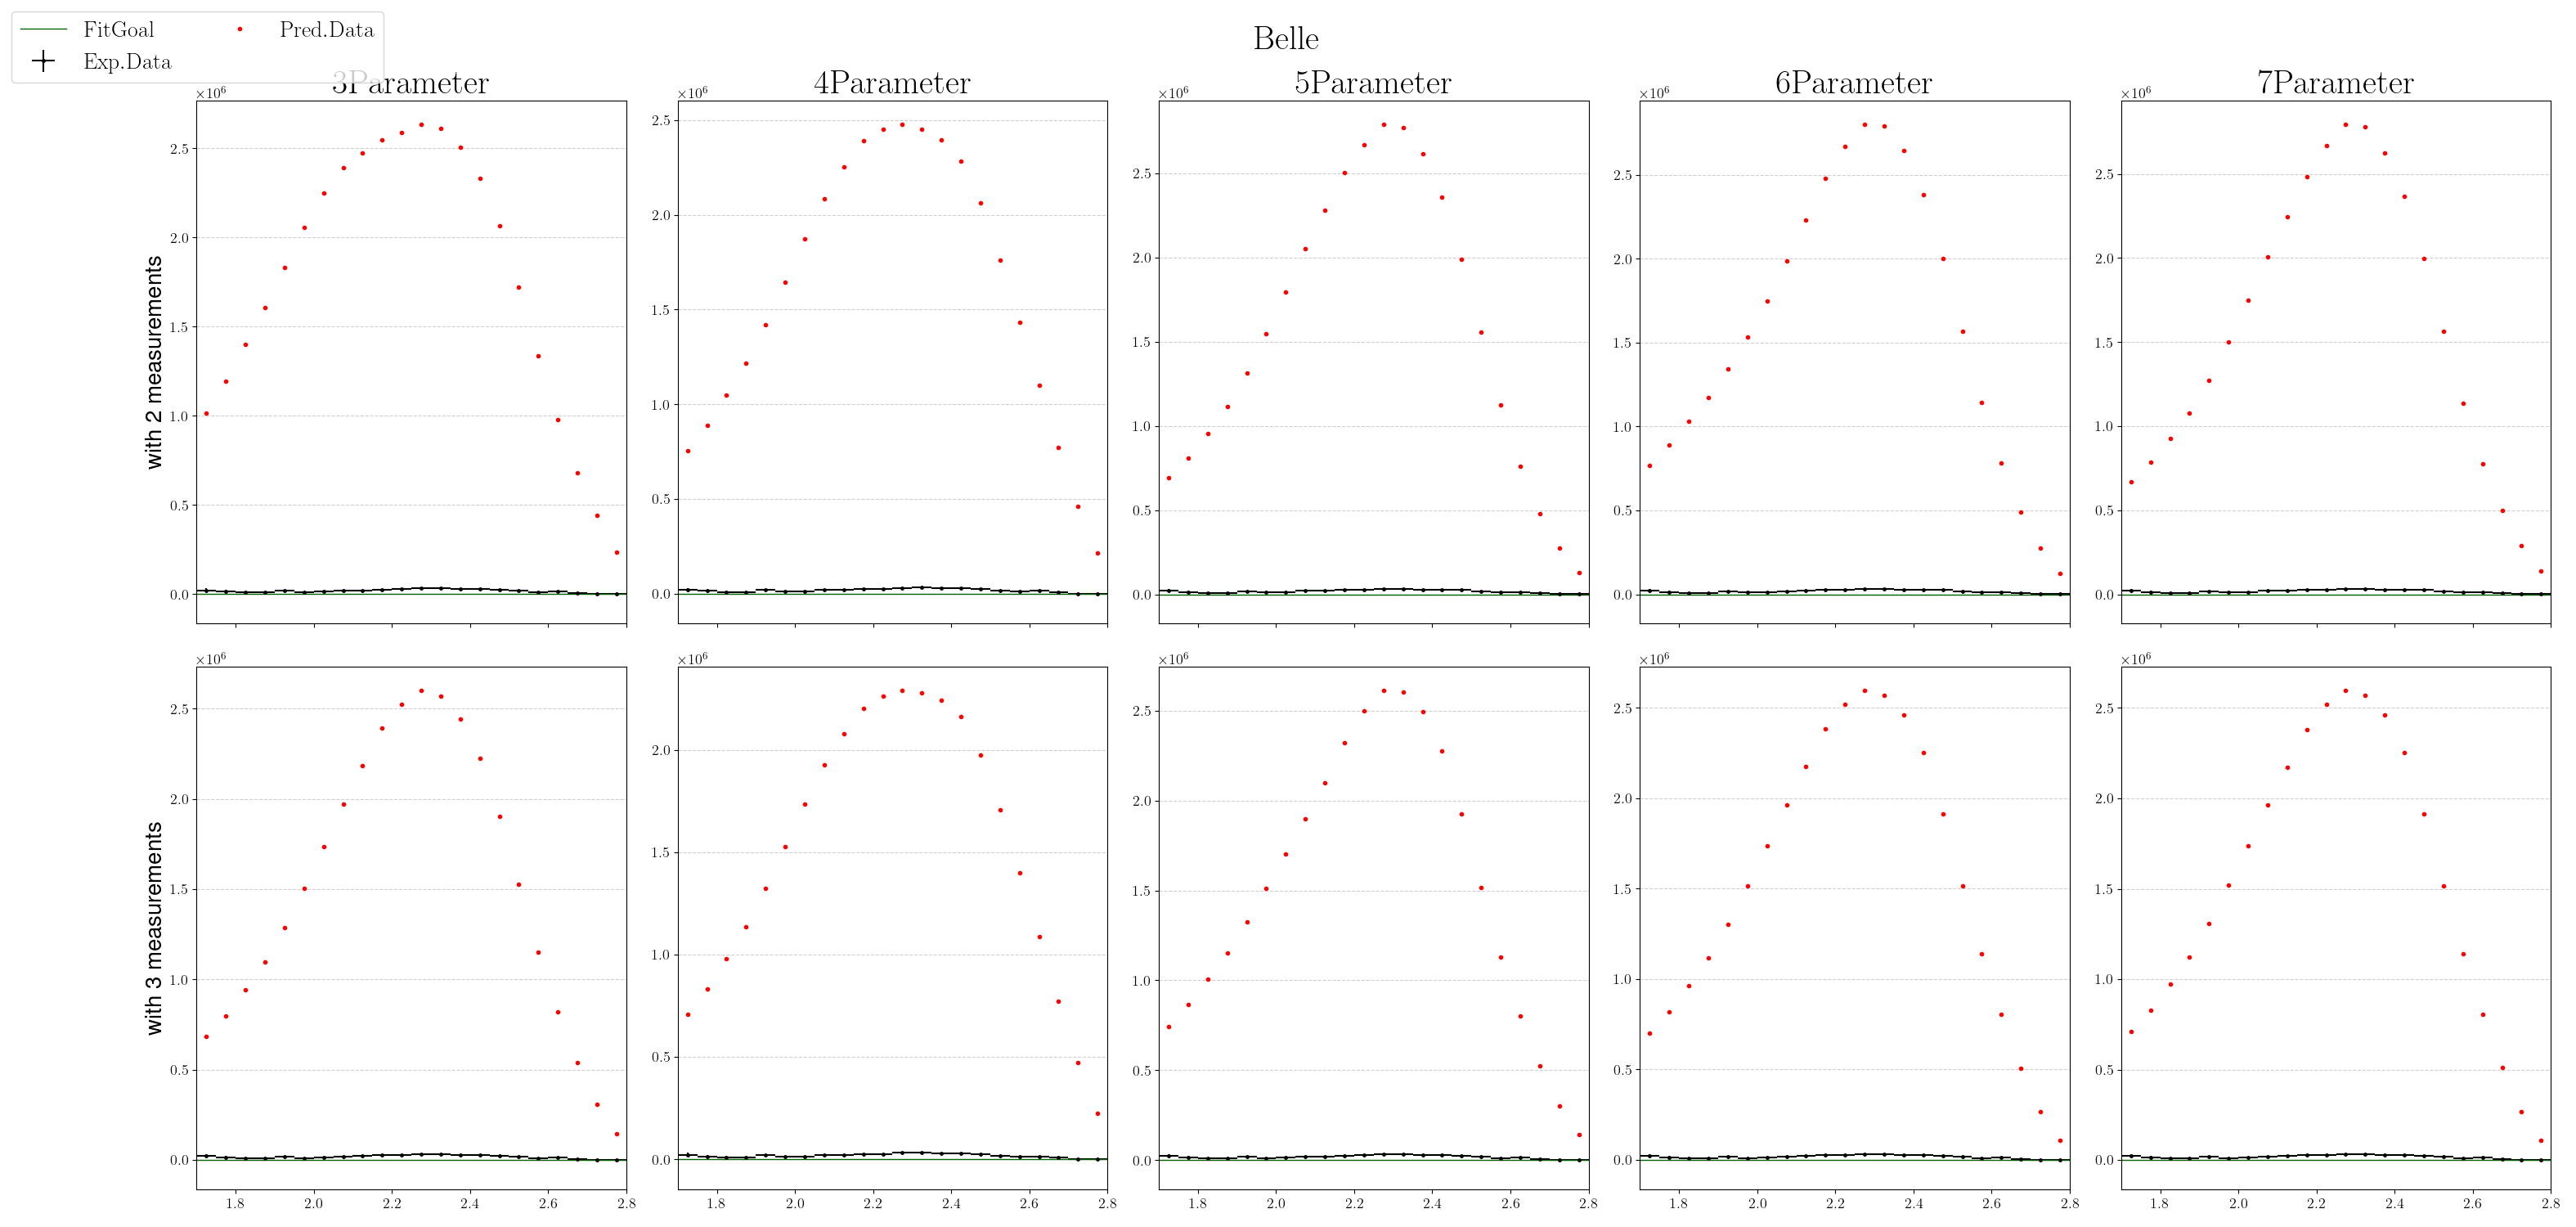
\includegraphics[scale=0.3]{../compare/belle_soft_compare.png}
    \caption{Fit Comparison for 'belle'}
\end{figure}

\subsection{Just Babar semileptonic}
The fit for \textit{'babar\_sem'} looked off in the previous plots, even though the $\chi^2$ was low. So I fitted only using the data from \textit{'babar\_sem'}. As you can see in the following,
the fit is not good, while for \textit{'babar\_hadtag'} and \textit{'babar\_incl'} it works quiet well, there could be a problem with the input I'm giving the fit for \textit{'babar\_sem'}.
\begin{figure}[H]
    \centering
    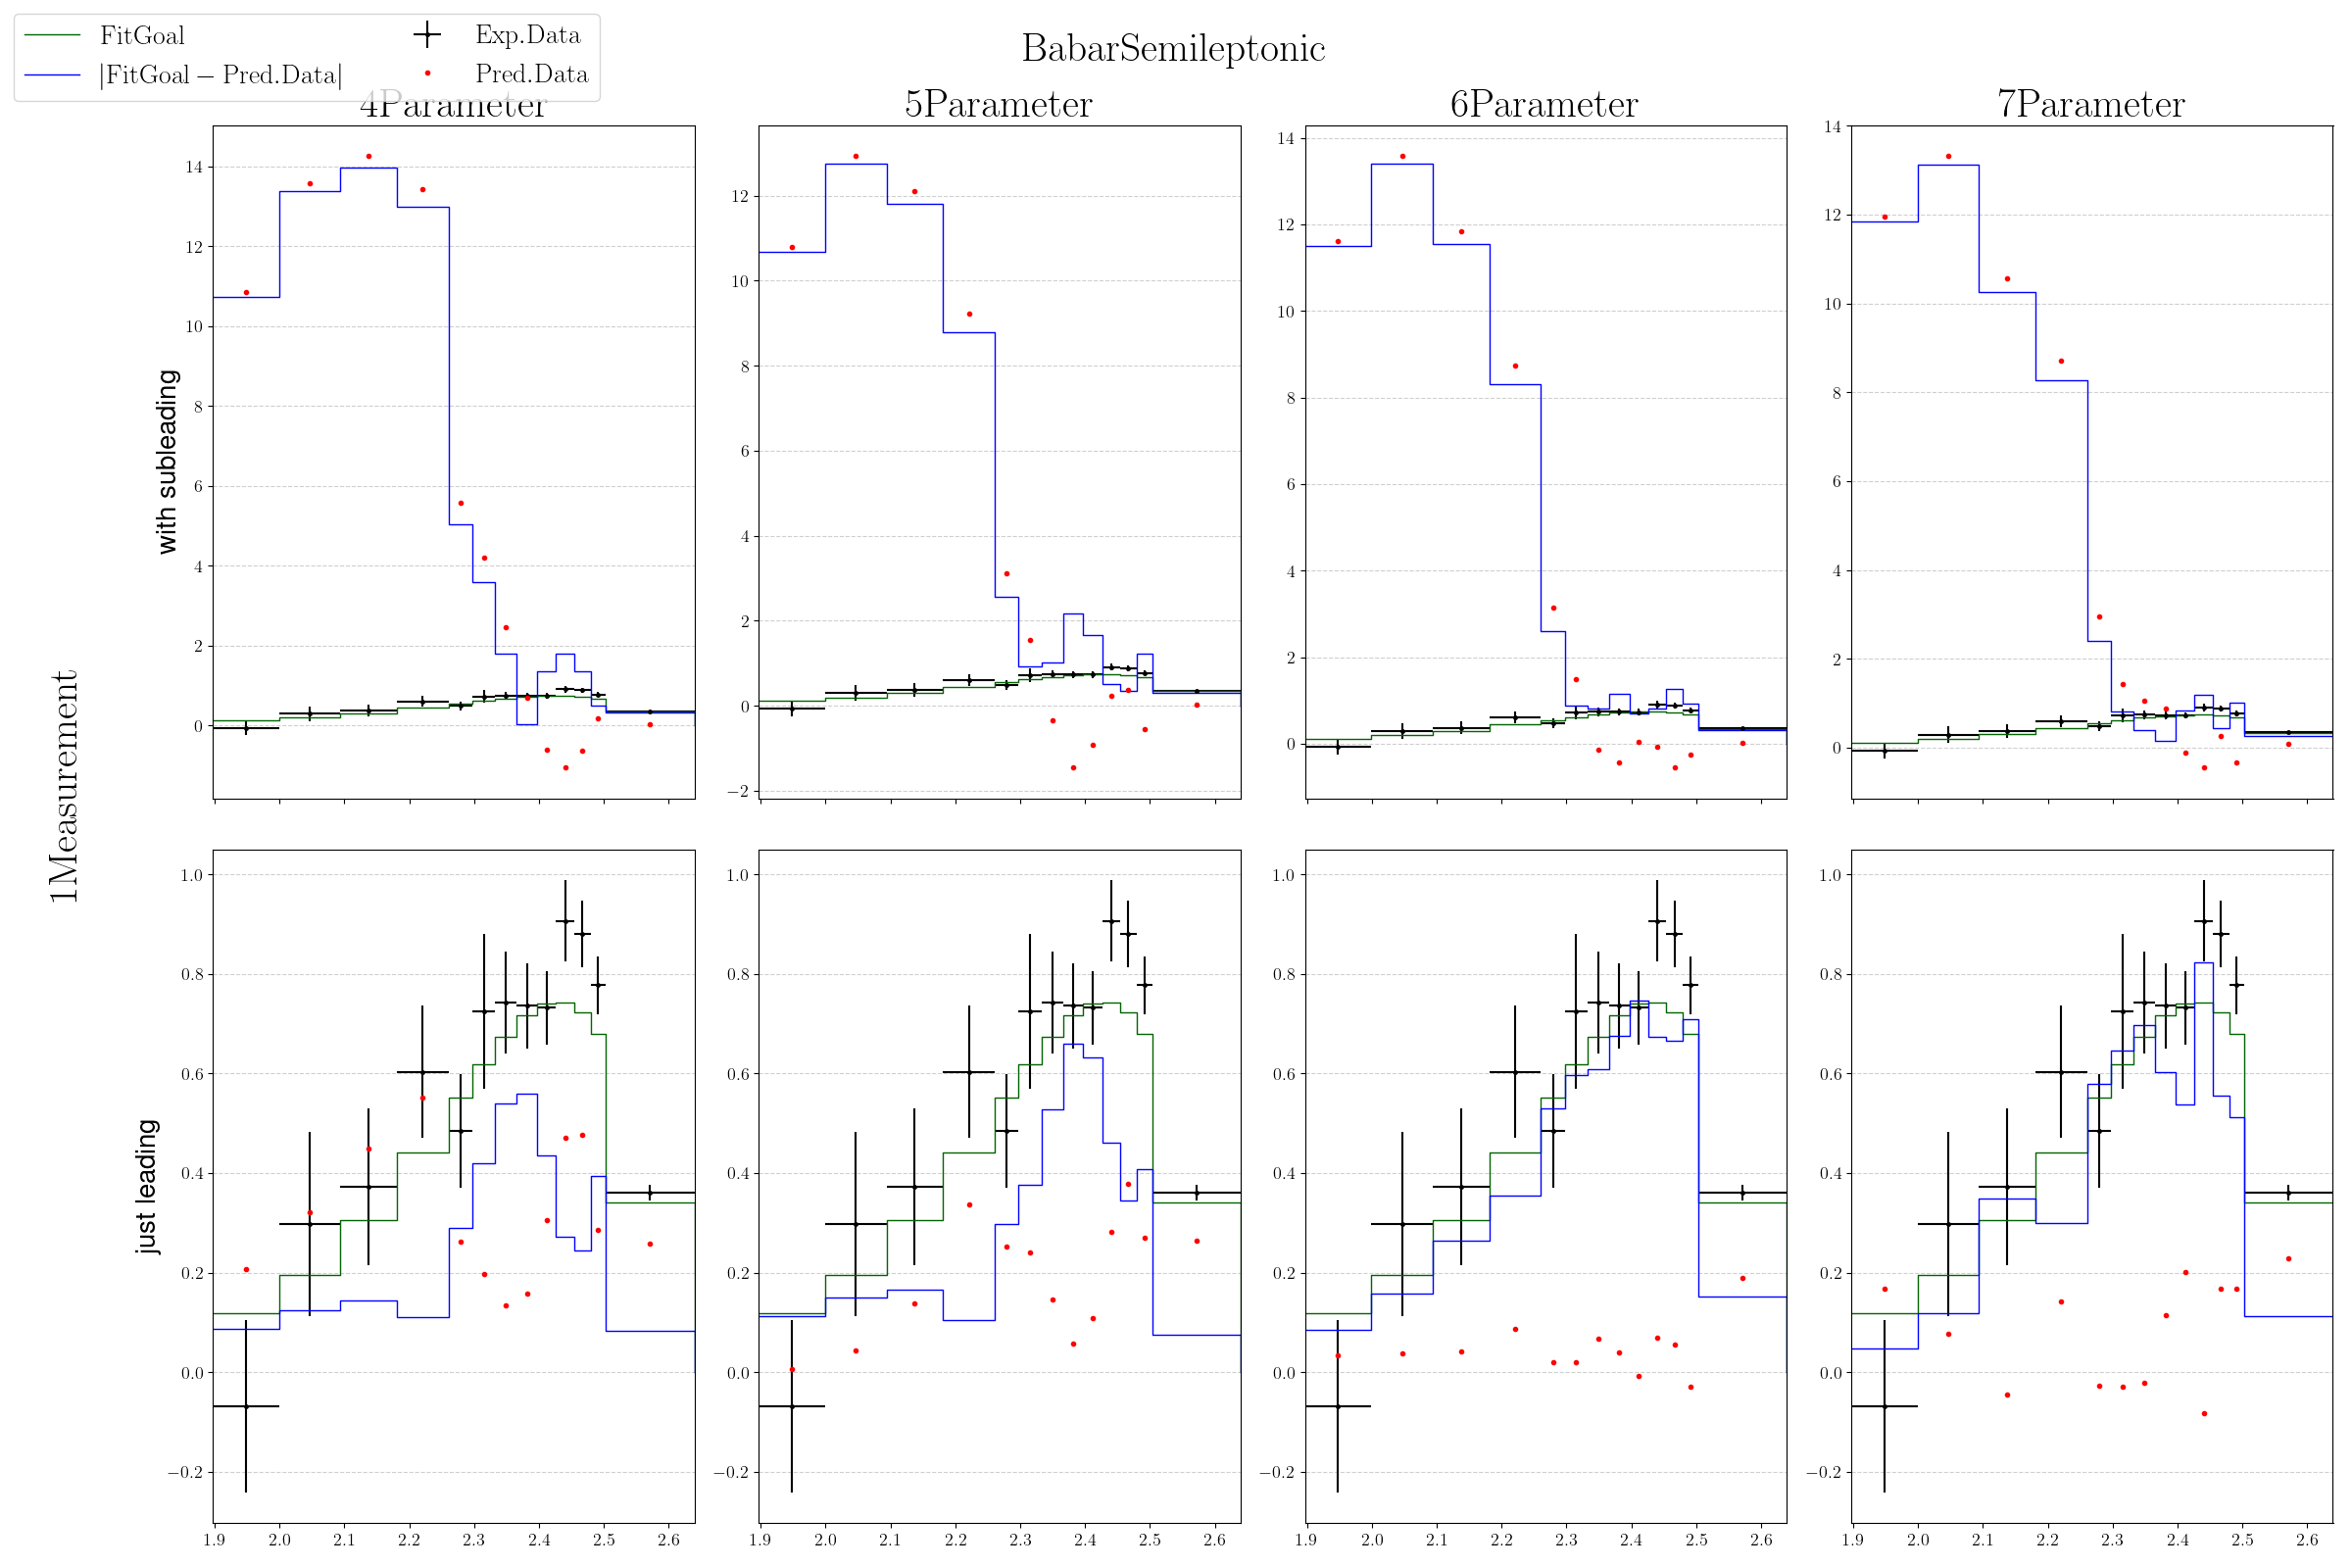
\includegraphics[scale=0.3]{../compare/just_babar_sem.png}
    \caption{Fit Comparison while using just the data from \textit{'babar\_sem'}}
\end{figure}

\begin{table}[H]
    \begin{tabular}{|p{3.5cm}|p{3.5cm}|p{3.5cm}|l|l|l|}
        \hline
        Number of included measurements & With or without subleading theory & Number of fitted parameters & $\chi^2$ & $m_b$ [\unit{GeV}] & $a_0$ (Norm) \\
        \hline
        1&subleading&4&25004.71&4.6698&0.9373\\
        1&subleading&5&19358.95&4.6747&0.9563\\
        1&subleading&6&17826.66&4.6622&0.9707\\
        1&subleading&7&15242.57&4.6587&0.9786\\
        1&leading&4&116.98&3.9847&0.5392\\
        1&leading&5&150.55&4.0966&0.6603\\
        1&leading&6&237.47&4.0095&0.0095\\
        1&leading&7&168.51&3.5833&0.5549\\
        \hline
        \hline
        Result from paper&&&&4.764&\\
        \hline 
    \end{tabular}
    \caption{Values calculated with the fit-parameters just using \textit{'babar\_sem'}}
\end{table}

\begin{table}[H]
    \begin{tabular}{|l|l|l|l|l|l|l|l|l|l|l|}
        \hline
        $n_{meas}$&&$n_{pars}$&$c_0$ & $c_1$& $c_2$ & $c_3$ & $c_4$ & $c_5$ & $c_6$\\
        \hline
        1&s&4&0.931&-0.361&0.053&0.025\\
        1&s&5&0.905&-0.382&0.130&0.112&0.073\\
        1&s&6&0.885&-0.401&0.128&0.163&0.101&0.044\\
        1&s&7&0.874&-0.411&0.108&0.119&0.186&0.063&0.056\\
        1&l&4&0.000&0.870&0.492&-0.029\\
        1&l&5&0.000&0.856&0.476&-0.202&-0.004\\
        1&l&6&0.077&0.669&0.224&-0.277&-0.552&-0.339\\
        1&l&7&0.000&-0.178&-0.780&-0.554&-0.209&-0.060&-0.070\\
        \hline
    \end{tabular}
    \caption{$c_n$ calculated by $a_n$ which are the fitted parameters using only data from \textit{'babar\_sem'}}
\end{table}

\section{Open Questions}

\begin{enumerate}
    \item What is $d_2$ in the subleading theory and what values has it?
    \item Something is off with \textit{'babar\_sem'}, how can I fix it?
\end{enumerate}

\end{document}